% This must be in the first 5 lines to tell arXiv to use pdfLaTeX, which is strongly recommended.
% \pdfoutput=1
% In particular, the hyperref package requires pdfLaTeX in order to break URLs across lines.

\documentclass[11pt]{article}

% Remove the "review" option to generate the final version.
\usepackage{acl}

% Standard package includes
\usepackage{times}
\usepackage{latexsym}

% For proper rendering and hyphenation of words containing Latin characters (including in bib files)
\usepackage[T1]{fontenc}
% For Vietnamese characters
% \usepackage[T5]{fontenc}
% See https://www.latex-project.org/help/documentation/encguide.pdf for other character sets

% This assumes your files are encoded as UTF8
\usepackage[utf8]{inputenc}

% This is not strictly necessary, and may be commented out,
% but it will improve the layout of the manuscript,
% and will typically save some space.
\usepackage{microtype}

% If the title and author information does not fit in the area allocated, uncomment the following
%
%\setlength\titlebox{<dim>}
%
% and set <dim> to something 5cm or larger.

% ceci's custom
\usepackage{amsmath,amsthm,amsfonts,amssymb,amscd}
\usepackage{mathrsfs}
\usepackage{times}
\usepackage{graphicx} % 插入图像
\usepackage{wrapfig}
\usepackage{subcaption}
\usepackage{multirow}


% \title{Constrain the Relational Dimensions with Conjugation for \\ Complex Knowledge Graph Embeddings}
\title{Parameters Conjugation for Knowledge Graph Embeddings \\ in Complex Space}
% elegant = simple and clear

\author{
  Xincan Feng\textsuperscript{\dag \ddag}, Zhi Qu\textsuperscript{\dag}, Yuchang Cheng\textsuperscript{\ddag}, Taro Watanabe\textsuperscript{\dag}, Nobuhiro Yugami\textsuperscript{\ddag} \\
  \textsuperscript{\dag}Natural Language Processing Laboratory, Nara Institute of Science and Technology \\
  % 8916-5 Takayamacho, Ikoma, Nara, Japan \\
  \textsuperscript{\ddag}Multilingual Knowledge Computing Laboratory, Fujitsu Ltd. \\
  % 4-1-1 Kamikodanaka, Nakahara Ward, Kawasaki, Kanagawa, Japan \\
  \texttt{\{feng.xincan.fy2, qu.zhi.pv5, taro\}@is.naist.jp} \\
  \texttt{\{cheng.yuchang, yugami\}@fujitsu.com}\\
  }

% Author information can be set in various styles:
% For several authors from the same institution:
% \author{Author 1 \and ... \and Author n \\
%         Address line \\ ... \\ Address line}
% if the names do not fit well on one line use
%         Author 1 \\ {\bf Author 2} \\ ... \\ {\bf Author n} \\
% For authors from different institutions:
% \author{Author 1 \\ Address line \\  ... \\ Address line
%         \And  ... \And
%         Author n \\ Address line \\ ... \\ Address line}
% To start a seperate ``row'' of authors use \AND, as in
% \author{Author 1 \\ Address line \\  ... \\ Address line
%         \AND
%         Author 2 \\ Address line \\ ... \\ Address line \And
%         Author 3 \\ Address line \\ ... \\ Address line}

% \footnote{\url{http://acl-org.github.io/ACLPUB/formatting.html}}

% \begin{quote}
% \begin{verbatim}
% \documentclass[11pt]{article}
% \end{verbatim}
% \end{quote}

% \footnote{This is a footnote.}

% \begin{table}
% \centering
% \begin{tabular}{lc}
% \hline
% \textbf{Command} & \textbf{Output}\\
% \hline
% \verb|{\"a}| & {\"a} \\
% \verb|{\aa}| & {\aa}  \\\hline
% \end{tabular}
% \begin{tabular}{lc}
% \hline
% \textbf{Command} & \textbf{Output}\\
% \hline
% \verb|{\c c}| & {\c c} \\ 
% \verb|{\u g}| & {\u g} \\ 
% \hline
% \end{tabular}
% \caption{Example commands for accented characters, to be used in, \emph{e.g.}, Bib\TeX{} entries.}
% \label{tab:accents}
% \end{table}

% \begin{quote}
% \tt\verb|\pdfendlink| ended up in different nesting level than \verb|\pdfstartlink|.
% \end{quote}

% \begin{table*}
% \centering
% \begin{tabular}{lll}
% \hline
% \textbf{Output} & \textbf{natbib command} & \textbf{Old ACL-style command}\\
% \hline
% \citep{Gusfield:97} & \verb|\citep| & \verb|\cite| \\
% \citealp{Gusfield:97} & \verb|\citealp| & no equivalent \\
% \citet{Gusfield:97} & \verb|\citet| & \verb|\newcite| \\
% \citeyearpar{Gusfield:97} & \verb|\citeyearpar| & \verb|\shortcite| \\
% \hline
% \end{tabular}
% \caption{\label{citation-guide}
% Citation commands supported by the style file.
% The style is based on the natbib package and supports all natbib citation commands.
% It also supports commands defined in previous ACL style files for compatibility.
% }
% \end{table*}


% Contents
% 介绍背景知识:
    % 知识图谱
    % KGC、link prediction task和KGE model
% 介绍方法思路:
    % 从复数、双曲等模型中得到灵感
    % 介绍对比模型,解释方法
% 介绍实验设置:
    % 解释自己模型的预想问题和辅助实验:
        % 猜测1:这种方法也不是随便哪个维度都可以,因此设置了其它维度的对比实验
        % 猜测2:这种方法的缺陷可能是参数的regulization,因此设置了-reg的对比实验
    % 介绍实验设备、参数选择、数据集:
        % 统一GPU
        % ComplEx选择了最佳参数,5StarE选择了一致参数进行多组实验
        % 采用了标准的5个数据集,包括最大的数据集
% 分析结果、方法优缺点:
    % 统计结果:
        % 5StarE,ComplEx,不同位置,-reg结果
        % 结果的t-test比较,是否属于同一分布
        % 实证确定结论:我们提出的方法是有以下三个优点的,其次确定我们的方法必须选择对位置,以及使用此法可能产生的问题(优点)
    % 分析优点:
        % 简化计算,近似相同表现(用理论计算过程+实验结果所需时间+实验t-test+实验mrr图+output图+数据集relation统计说明)!!
        % 美化视觉(用理论计算过程+理论3D图说明)
        % 泛用性(用自己的思考+实验结果说明)
    % 分析缺点:
        % 在小数据集上可能会表现下降(用learning curve+-reg实验+output图+数据集relation统计说明,回答为何会下降)!!
% 总结:
    % 方法如何使用:在复数KGE模型中选择合适位置进行共轭(注意根据模型不同,不是所有位置效果都一样)
    % 方法效果:这是一个拥有xx优点的方法,虽然在xx时可能会出现问题,但在大数据集上性能较好,且具有一定的泛化性,具有实用价值。

% 后续修改:
    % 数学公式加ref编号
    % 参考文献整理
    % abstract --> 课题最重要、再描述、解决方法稍微少些可以,现在研究中视觉化重要吗?
    % visualization --> 对比最后的视觉效果重要吗?better --> regular? explainable 或者只放在实验部分稍微提一些,不要写在contribution里。
    % datasets reduce to three, two addition如果有用再用,没有用就不用

\begin{document}
\maketitle
\begin{abstract}
Knowledge Graph Embedding (KGE) have been a popular approach to do link prediction task for Knowledge Graph Completion (KGC).
Researchers are designing increasingly complicated models to improve model expressiveness.
We need to simplify the models without losing performance.
Besides, many Knowledge Graph (KG) applications like (https://aclanthology.org/2021.acl-demo.14.pdf) regard visual appeal as important, where appropriate visuals can better convey the points of the data and facilitate user interaction.
Our research proposed parameters conjugation ———— a dimension-level restriction method, to reduce computation to at most 50\% and help obtain better visualization while receiving comparable performance in most cases in the complex number represented KGE models.
We verified our method's generalizability in two best KGE models: $5^{\bigstar}\mathrm{E}$
\hyperlink{Nay21}{(Nayyeri et al. 2021)}
\cite{Nayyeri_Vahdati_Aykul_Lehmann_2021}
and $\mathrm{ComplEx}$
\hyperlink{Tro16}{(Trouillon et al. 2016)}.
\end{abstract}

\section{Introduction}
Knowledge Graph (KG) has become trustable information source in applications including question answering, data integration, recommender systems 
\hyperlink{JiS20}{(Ji et al. 2020)} and automated personal agents
\hyperlink{Tro16}{(Trouillon et al. 2016)}.
Knowledge Graph (KG) is the directed graphical Knowledge Base (KB) representation in the form of (head, relation, tail) triples.
The heads and tails in KG triples are also called the entities, and the relations are correspondingly called the links that relate the entities.
In the graph representation of KG, entities are usually represented as nodes, and links are represented as edges.
From a mathematical point of view, entities and links are often represented as vectors and transformation functions, respectively, in Knowledge Graph Embedding (KGE) models.

KGE is a prominent approach used for Knowledge Graph Completion (KGC) by predicting missing links
\hyperlink{Nay21}{(Nayyeri et al. 2021)}.
We do KGC because, in addition to the existing triples, KGE models can learn missing links that indicate implicit relations among heads and tails in the KG.
Link Prediction task is one of the main problems in Statistical Relational Learning (SRL, Getoor and Taskar, 2007).
KGC extends KG's applicability by saving repetitive human labor for constructing KBs.

KGE models usually define a specific represention, and use a transformation function to map entities (nodes) through links (edges) into a corresponding vector space, and then calculate the plausibility of triples via a corresponding score function
\hyperlink{Nay21}{(Nayyeri et al. 2021)}.
Thus, the main directions in improving the KGE models are: representations, vector spaces, and transformation functions.
We generically concluded the following about above three directions:

\begin{itemize}
\item Compared with real number representation, the composition of complex number can handle a larger variety of relations, among them symmetric and antisymmetric relations
\hyperlink{Tro16}{(Trouillon et al. 2016)}.

\item Compared with Euclidean space, the Hyperbolic space models can save more structures using fixed or trainable curvatures in different positions for hierarchical relations
\hyperlink{Cha20}{(Chami et al. 2020)}.

\item Compared with naive addition or multiplication transformation functions, more specific designed functions, including projective geometric functions, 
support multiple simultaneous transformations, and are more capable to represent multiple structures in multi-relational KGs
\hyperlink{Nay21}{(Nayyeri et al. 2021)}.
\end{itemize}

The relationship among transformation functions, representation methods and dimensions are that:
The transformation functions distinguish the extent to which the KGE model is able to learn complicated patterns formed by combinations of entities and links
\hyperlink{Nay21}{(Nayyeri et al. 2021)}.
The representation methods of different vector spaces are where the transformation functions built with.
Dimensions are the base of the representation methods and can thus nail the transformation functions' capabilities.
From above, we noticed two points:

\begin{itemize}
\item The increased performance from real number to complex number representation, which enables the imaginary and real part dimensions to be relational, indicates the benifit of \textbf{hidden relation} among parameter dimensions.

\item The increased performance from Euclidean space to Hyperbolic space, which enables the distances or angles of \textbf{different positions} to vary in different degrees, indicates different positions in the parameter dimensions could have different degrees of freedom. 
\end{itemize}

Here was born our intuition that the dependent parameter dimensions are maybe capable enough compared with independent dimensions to do KGE. 
Since, although the KGE models have kept on discovering more complex transformations, the relationship between the transformation complexity and the model expressiveness is sophisticated.
Using conjugation on complex number is a natural thought.

Our contribution is that we proposed the parameters conjugation method, i.e. a dimension-level restriction method used in the complex number represented KGE models.
Specifically, our method formulates conjugated parameters in appropriate dimensions of the transformation functions, so that to reduce parameter size and computation.
Although the origin models can be different, using our method will more or less reduce the computation.
Experiments demonstrated that our conjugated models usually receive comparable performance as the origin models under the same hyperparameters settings.
We verified our method's generalizability in two best performing KGE models: $5^{\bigstar}\mathrm{E}$
\hyperlink{Nay21}{(Nayyeri et al. 2021)} and $\mathrm{ComplEx}$
\hyperlink{Tro16}{(Trouillon et al. 2016)}.
Besides, because our method creates stronger geometric restriction on nodes and edges, it also obtains better visualization of the KGs than the origin models by making the generated KGs clearer.

The remainder of the paper is organized as follows:
We first formulated our parameters conjugation method in two baseline models, call our conjugate models $\mathrm{complexC}$ and $5^{\bigstar}\mathrm{Ce}$.
We then describe experiments on large scale public benchmark datasets, in which we empirically show that our method not only reduces computation, but also brings better visualization for KG applications.

To compare our method's limitations with original approaches using only half of the parameters, we also did auxiliary experiments to see how the original models would perform with only half of the parameters in the regularization term. 
This should help practitioners when applying our method to more datasets.

\section{Related work}
KGE models can be classified in many ways. 
Our method involves both the representation and the dimensional position of the model. 
We describe the classification according to the representation methods, and the classification according to the vector spaces, that has inspired our method, and the related work under these two classifications.

KGE models that are classified according to their representation methods:

\textbf{Real Embeddings} Translation approaches include $\mathrm{TransE}$ 
\hyperlink{Bor13}{(Bordes et al. 2013)} 
and its variants 
(\hyperlink{Jie15}{Ji et al. 2015}, 
\hyperlink{Lin15}{Lin et al. 2015}).
Although these models are fairly simple and have few parameters, they fail to encode important logical properties (e.g., translations can't encode symmetry).

\textbf{Complex Embeddings} $\mathrm{ComplEx}$ 
\hyperlink{Tro16}{(Trouillon et al. 2016)} gives a clear comparison with respect to existing approaches using only real numbers by presenting an equivalent reformulation of their model that involves only real embeddings.
$\mathrm{RotatE}$ 
\hyperlink{Sun19}{(Sun et al. 2019)} does require additional optimization component to effectively draw negative samples for training.
$5^{\bigstar}\mathrm{E}$ 
\hyperlink{Nay21}{(Nayyeri et al. 2021)}
uses Möbius transformation as the transformation function, which is the composition of four functions that can represent five transformations. 

KGE models that are classified according to their vector spaces:

\textbf{Euclidean Embeddings} Tensor factorization methods such as $\mathrm{RESCAL}$ 
\hyperlink{Nic11}{(Nickel et al. 2011)} and $\mathrm{DistMult}$ 
\hyperlink{Yan15}{(Yang et al. 2015)}
are designed based on element-wise multiplication of transformed head and tail. 
In this case, the plausibility of triples is measured based on the angle of transformed head and tail.

\textbf{Non-Euclidean Embeddings} $\mathrm{MuRP}$ 
\hyperlink{Bal19}{(Balazevic et al. 2019)}
minimizes hyperbolic distances between a re-scaled version of the head entity embedding and a translation of the tail entity embedding. 
It uses hyperbolic embeddings with fewer dimensions than its Euclidean analogues.
$\mathrm{ATTH}$ 
\hyperlink{Cha20}{(Chami et al. 2020)}
leverages trainable hyperbolic curvatures per relationship to simultaneously capture logical patterns and hierarchies.
However, it also needs optimization methods in tangent space (i.e., Euclidean).

\section{Method}
Our method turns half of the transformation function parameters into the complex conjugate; 
the position selection of the conjugated parameters depends on the original model.
Complex embeddings set relational restriction for entities and links representation.
Our method further adds relational restriction within the transformation function parameters.

\subsection{Method Formulation}
$a,b,c,d \in \mathbb{C}$ are the parameters in the relation embedding matrices, also the transformation functions, 
$x \in \mathbb{C}$ is the entity embedding,
$Re(x)$ is the real part of the complex number $x$,
$\overline{x}$ is the complex conjugate of $x$.

$\mathrm{ComplEx}$
\hyperlink{Tro16}{(Trouillon et al. 2016)} is the first and also one of the best performing complex embedding models in Euclidean space.
They discussed the problem of finding the best ratio between expressiveness and parameter space size as the keystone of KGE models.
They demonstrated that complex vectors can effectively capture antisymmetric relations while retaining the efficiency benefits of the dot product, that is linearity in both space and time complexity.
In this model, relations are represented as real part of low-rank normal matrices, and relation embeddings naturally act as weights on each latent dimension.
Geometrically, each relation embedding is an anisotropic scaling of the basis defined by the entity embeddings, followed by a projection onto the real subspace.

By using our method, the original model $\mathrm{ComplEx}$ is adapted to the conjugate model $\mathrm{complexC}$, where relations are represented as the real part of low-rank conjugate matrices.
Specifically, we set the original normal square relation embedding matrices 
$\begin{bmatrix}
    a\\
\end{bmatrix}$
to be half the normal parameters and the other half their conjugate parameters. I.e.
$\begin{bmatrix}
    a & \overline{a}\\
\end{bmatrix}$.
In this model, since each parameter position is of the same importance, the positions of the conjugate parameters can be set randomly.

$5^{\bigstar}\mathrm{E}$
\hyperlink{Nay21}{(Nayyeri et al. 2021)} is a novel complex embedding model in Non-Euclidean space.
They tackled the problem of multiple sub-graph structures in the neighborhood (e.g. combinations of path and loop structures).
Unlike the $\mathrm{ComplEx}$ model, they replaced the dot product with the Möbius function to project the entities into Non-Euclidean space, so that to support multiple simultaneous transformations. 
The Möbius function has several favorable theoretical properties and this model subsumes $\mathrm{ComplEx}$ in that it embeds entities in much lower ranks with better performance.
(But the authors haven't published the hyperparameters, and we failed to reproduce the same performance.)
However, $5^{\bigstar}\mathrm{E}$ is inferior to $\mathrm{ComplEx}$ because the calculation is more sophisticated and hence costs more time.

Our method transforms the original model $5^{\bigstar}\mathrm{E}$ into the conjugate model $5^{\bigstar}\mathrm{Ce}$, where relations are represented as the real part of low-rank conjugate matrices.
Specifically, we set the original normal square relation embedding matrices 
$\begin{bmatrix}
    a & b\\
    c & d\\
\end{bmatrix}$
to be half the normal parameters and the other half their conjugate parameters. I.e.
$\begin{bmatrix}
    a & b\\
    \overline{b} & \overline{a}\\
\end{bmatrix}$, or 
$\begin{bmatrix}
    a & b\\
    -\overline{b} & \overline{a}\\
\end{bmatrix}$.
In this model, different positions of the parameters play different roles, and the best conjugate positions are the principal and secondary diagonal positions.
Note that experiments showed that, the parameters conjugation or negative parameters conjugation method achieved the same accuracy. 
Negative parameters conjugation on this model is equivalent to restricting the original Möbius function to the unitary Möbius transformation.

\subsection{Transformation Analysis}
$\mathrm{ComplEx}$: $a\in \mathbb{C}$
\[
    x \rightarrow
    \begin{bmatrix}
        a
    \end{bmatrix}
    x
    \rightarrow
    ax
    \]

$\mathrm{complexC}$: $a,\overline{a} \in \mathbb{C}$
\[
    \begin{bmatrix}
        x_1 & x_2
    \end{bmatrix} 
    \rightarrow
    \begin{bmatrix}
        a & \overline{a}
    \end{bmatrix}
    \begin{bmatrix}
        x_1 & x_2
    \end{bmatrix}
    \rightarrow
    \begin{bmatrix}
        ax_1 & \overline{a}x_2
    \end{bmatrix}
    \]

$5^{\bigstar}\mathrm{E}$: $a,b,c,d\in \mathbb{C}$
\[
    x \rightarrow
    \begin{bmatrix}
        x\\
        1
    \end{bmatrix}
    \rightarrow
    \begin{bmatrix}
        a&b\\
        c&d\\
    \end{bmatrix}
    \begin{bmatrix}
        x\\
        1
    \end{bmatrix}
    \rightarrow
    \frac{ax+b}{cx+d} 
    \]

Möbius transformation $\vartheta$ is capable of performing five kinds of transformations simultaneously
because it combines five subsequent transformations:
$\vartheta=\vartheta_4 \circ \vartheta_3 \circ \vartheta_2 \circ \vartheta_1$.
Among them
$\vartheta_1=x+\frac{d}{c}$
(translation by $\frac{d}{c}$),
$\vartheta_2=\frac{1}{x}$
(inversion and reflection w.r.t. real axis),
$\vartheta_3=\frac{bc-ad}{c^2} x$
(homothety and rotation), and
$\vartheta_4=x+\frac{a}{c}$
(translation by $\frac{a}{c}$).

$5^{\bigstar}\mathrm{Ce}$: 
$c = \overline{b}, d = \overline{a}$
(Note that $c = -\overline{b}, d = \overline{a}$ works fine as well, and this forms a unitary Möbius transformation.)
\[
    x \rightarrow
    \begin{bmatrix}
        x\\
        1
    \end{bmatrix}
    \rightarrow
    \begin{bmatrix}
        a & b\\
        \overline{b} & \overline{a}\\
    \end{bmatrix}
    \begin{bmatrix}
        x\\
        1
    \end{bmatrix}
    \rightarrow
    \frac{ax+b}{\overline{b}x+\overline{a}} 
    \]

The five subsequent transformations turn into:
$c = \overline{b}, d = \overline{a}$
$\vartheta_1=x+\frac{\overline{a}}{\overline{b}}$
(translation by $\frac{\overline{a}}{\overline{b}}$),
$\vartheta_2=\frac{1}{x}$
(inversion and reflection w.r.t. real axis),
$\vartheta_3=\frac{b\overline{b}-a\overline{a}}{\overline{b}^2} x$
(homothety and rotation), and
$\vartheta_4=x+\frac{a}{\overline{b}}$
(translation by $\frac{a}{\overline{b}}$).

\begin{figure*}[h!]
    \centering
    \begin{subfigure}{.49\textwidth}
        \vspace{0.2cm}
        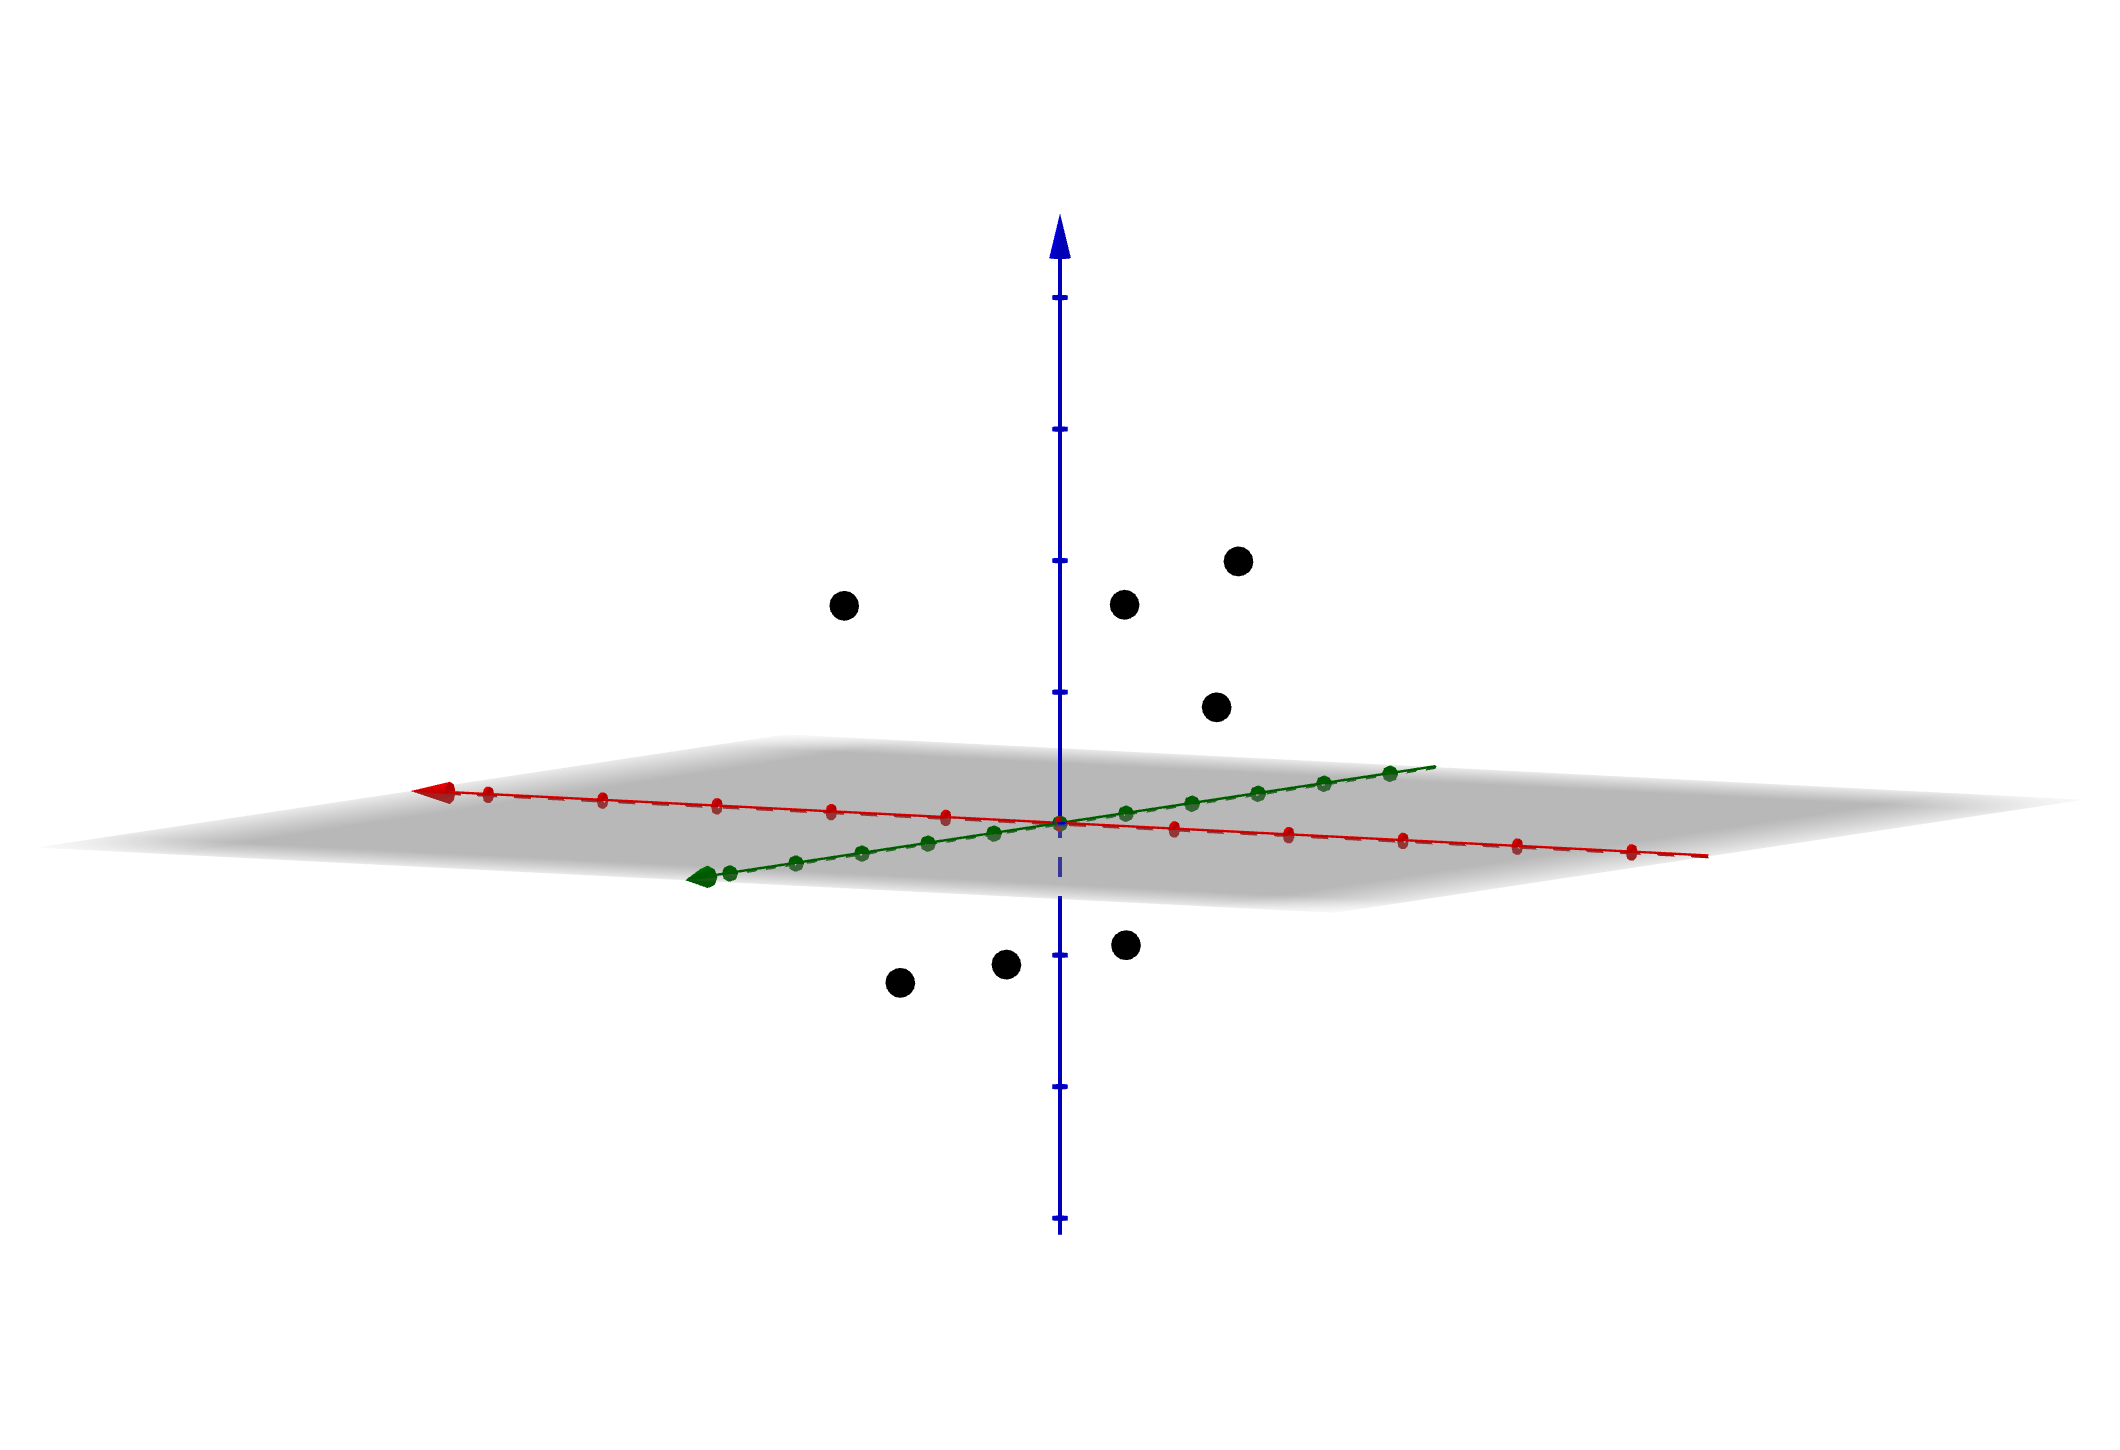
\includegraphics[scale=0.05]{figures/complex.png}
        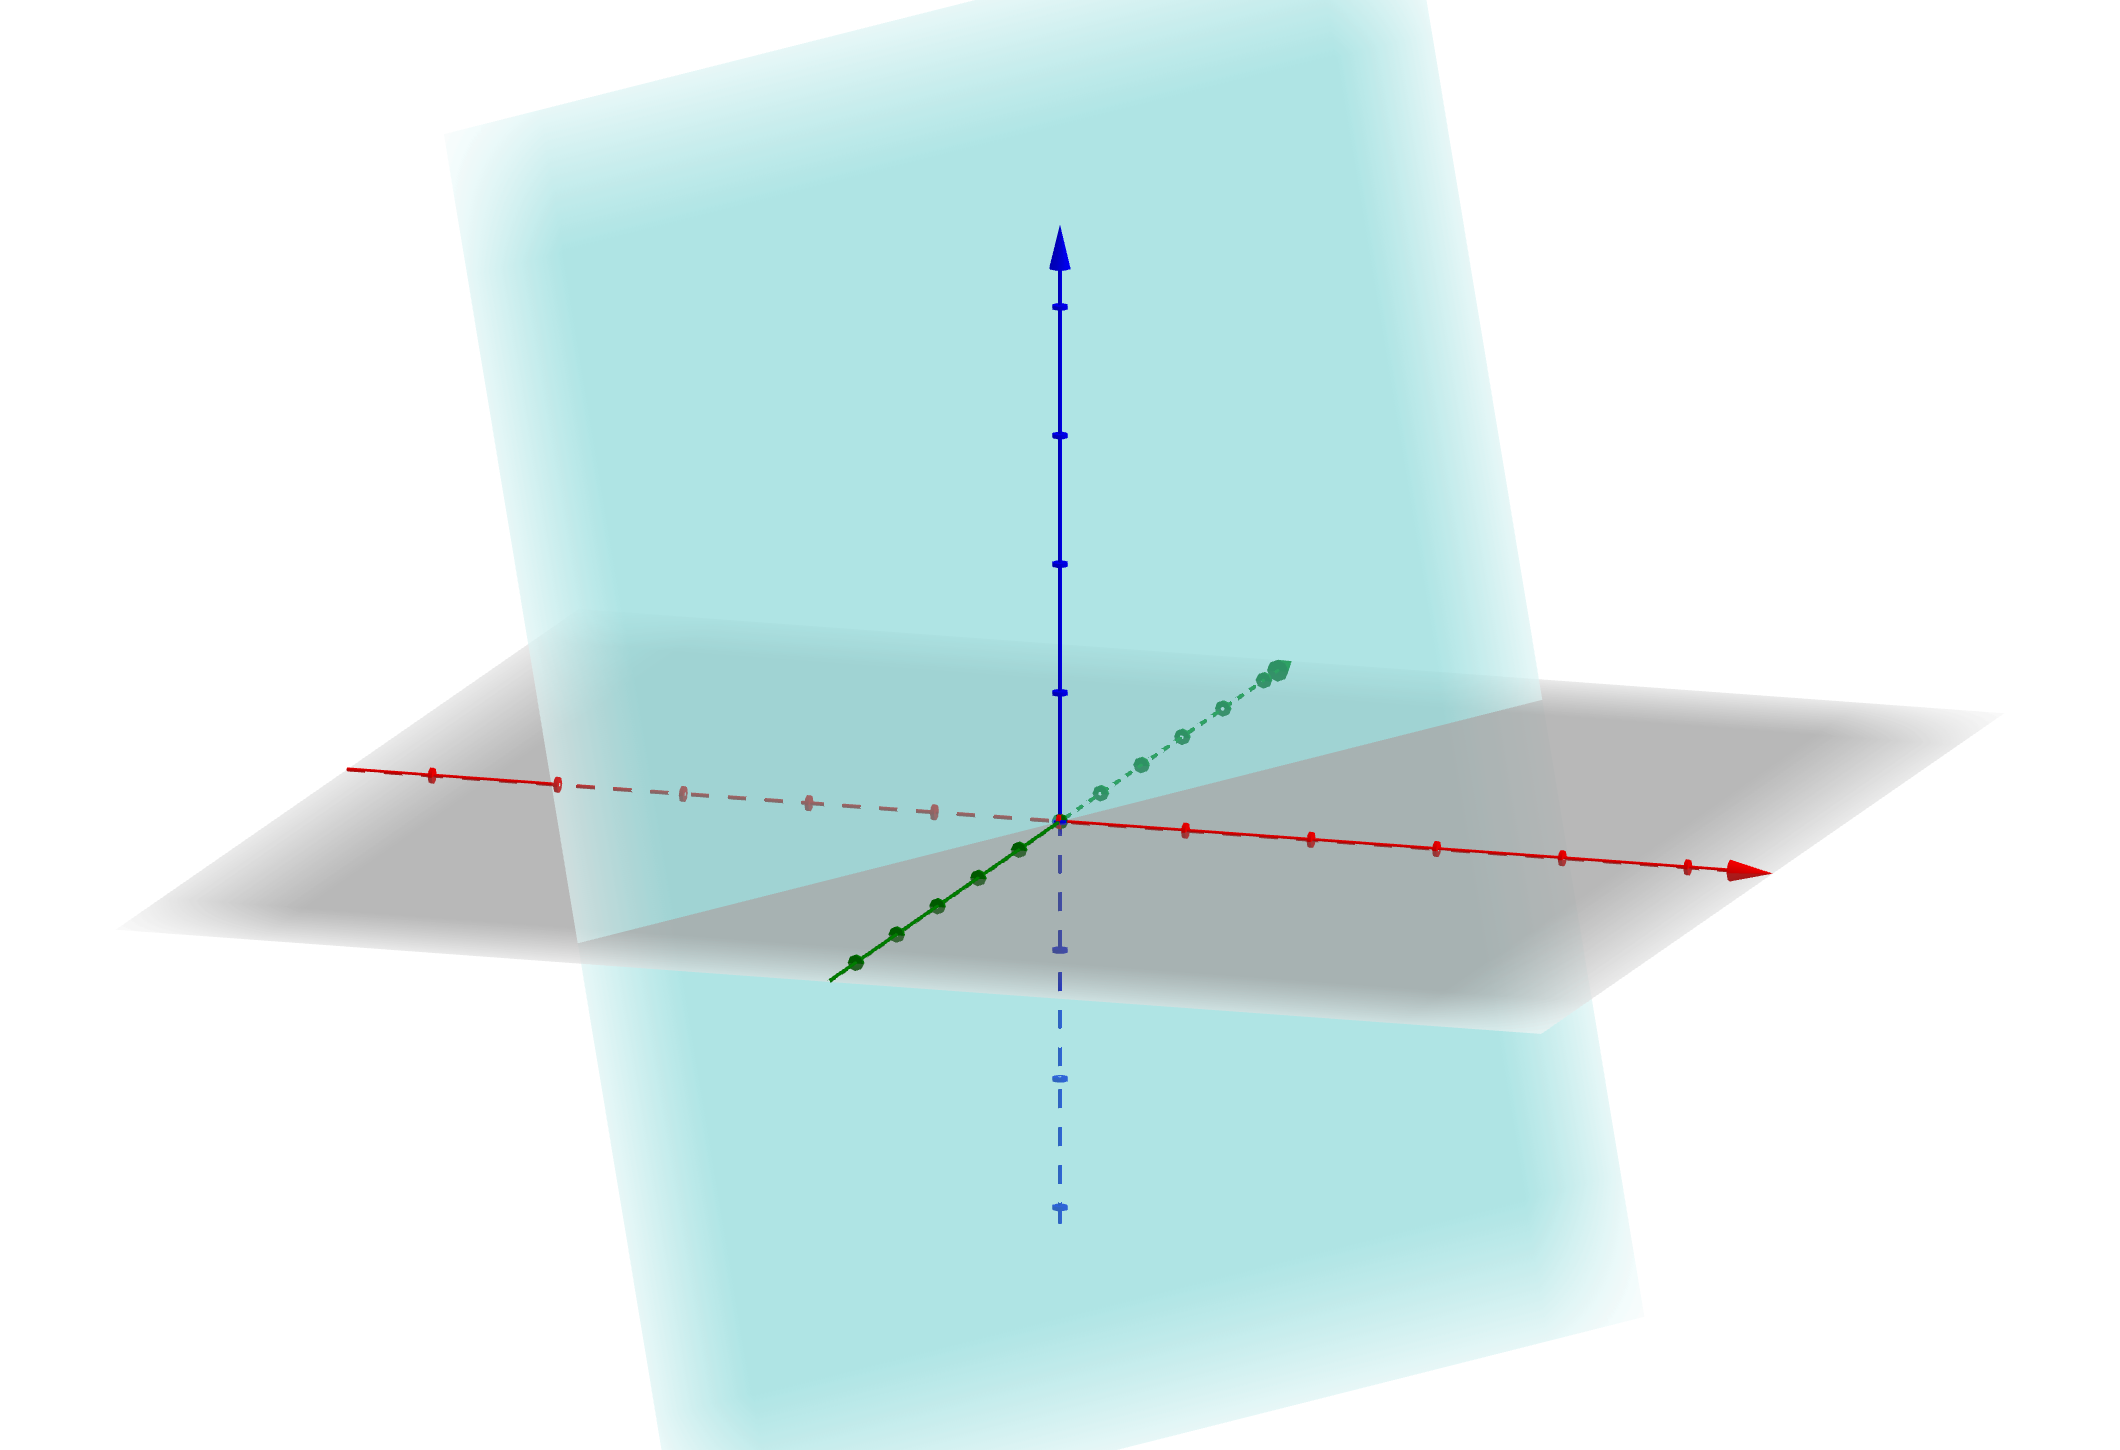
\includegraphics[scale=0.05]{figures/complexc.png}
        \vspace{0.2cm}
        \caption{
            Transformed entities by $\mathrm{ComplEx}$ and $\mathrm{complexC}$.
            The black points in the left graph are transformed entities. 
            In the original model, vector representations of the points are free in every dimension. 
            While in the conjugate model, half of the vector representations of the points are linearly dependent on the other half. 
            The linear relationship is illustrated in the right graph.}
    \end{subfigure}\hfill
    \begin{subfigure}{.49\textwidth}
        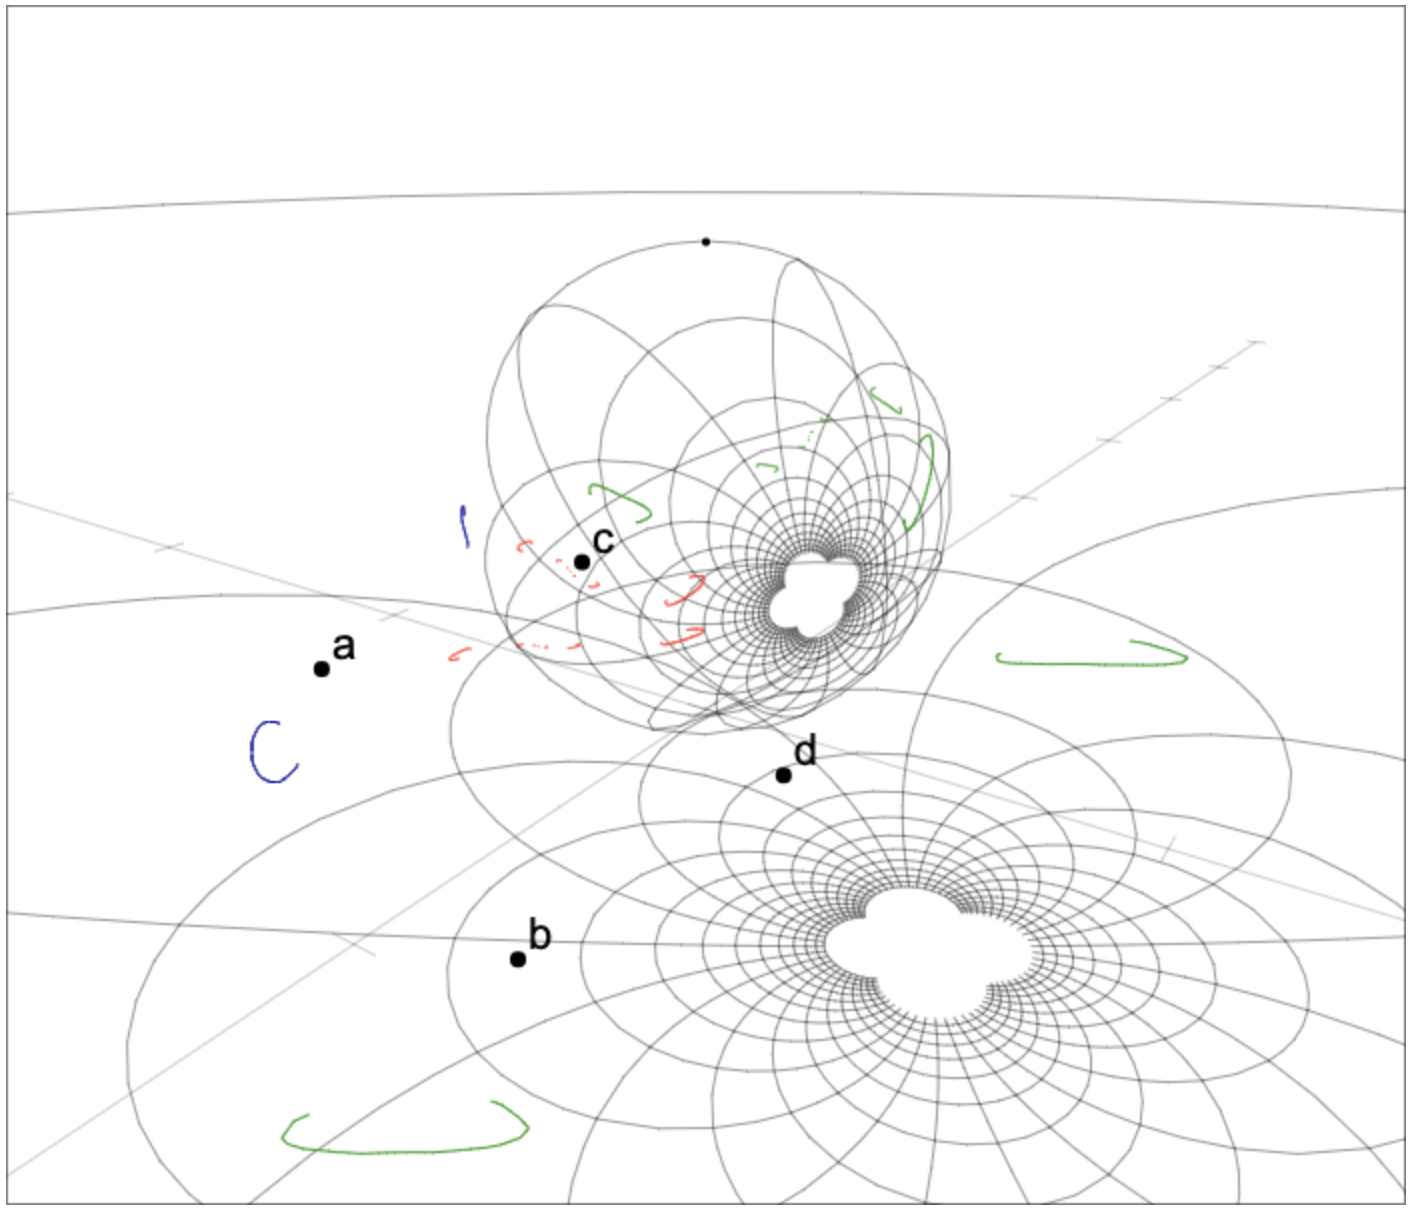
\includegraphics[scale=0.15]{figures/fivestare.png}
        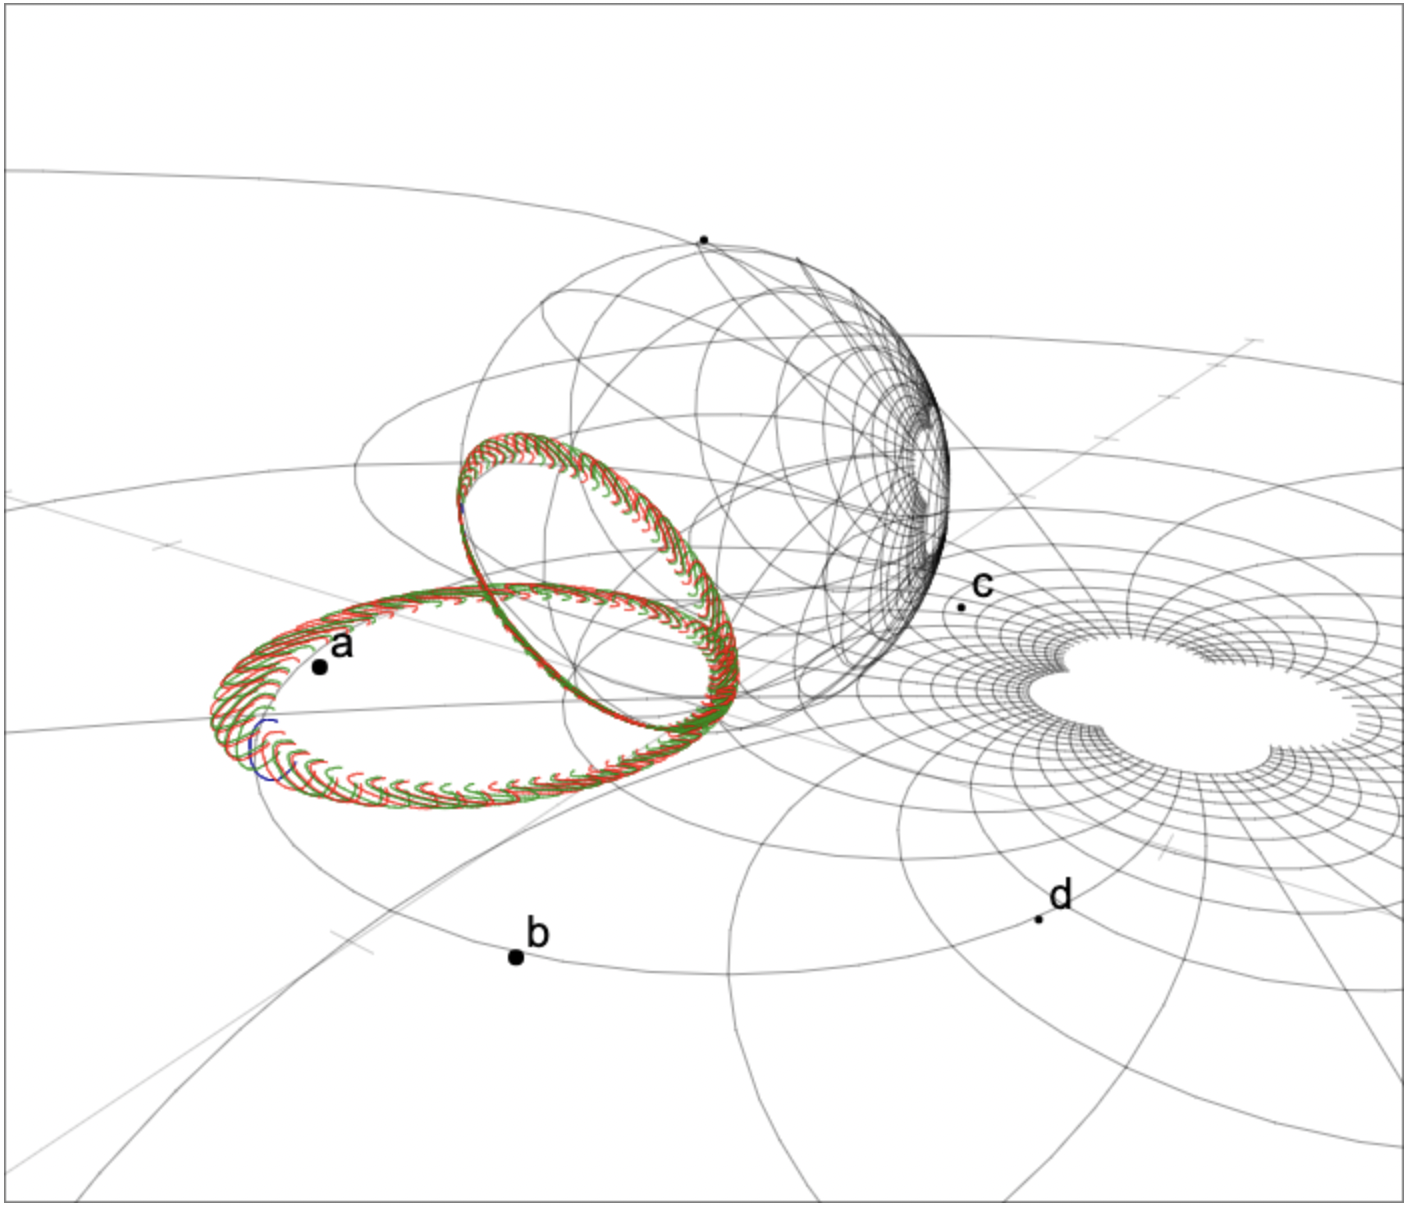
\includegraphics[scale=0.15]{figures/fivestarce.png}
        \caption{
            Transformed entities by $5^{\bigstar}\mathrm{E}$ and $5^{\bigstar}\mathrm{C^{-}e}$.
            The original model is shown on the left, and the negative conjugate model is shown on the right.
            Blue traces are the original entity and its projection in the Non-Euclidean space.
            Green traces are the multiple copies of the blue traces under iterations of the Möbius transformation.
            Red traces are the inverse of green traces.}
    \end{subfigure}
    \caption{Transformed entities illustrated in 3D
}
    
\end{figure*}\label{entities}

We conclude from above that: 

(i) The transformed entities in our conjugate models basicly retain the expressiveness for different relation patterns compared to their original ones.

(ii) The vector representations of transformed entities have more substantial geometric constraints (transformed entities are illustrated in Figure \ref{entities}).

\section{Experiments}
\subsection{Experimental Setup}
\textbf{Experiments Purposes}
To evaluate the performance of our method, and to explore potential problems and the reasons, we conducted the following comparison experiments.
(i) We experimented on five datasets to explore how the model performs on different datasets.
(ii) We experimented using different hyperparameter settings to explore whether hyperparameters influence our method.
(iii) We experimented with different conjugate dimensions to explore what kind of dimensions are more suitable for $5^{\bigstar}\mathrm{E}$. 
We set $c = -\overline{b}, d = \overline{a}$ in model $5^{\bigstar}\mathrm{C^{-}e}$.
And $c = \overline{a}, d = \overline{b}$ in model $5^{\bigstar}\mathrm{De}$.
(iv) We experimented where the regularization term is reduced to half of the parameters on the original model ($5^{\bigstar}\mathrm{E_{hreg}}$) to explore whether the flaw in our model is similar to the effect of reduced parameters.
We compared all experiments results running on GeForce GTX 1080 Ti,
except for the largest database YAGO3-10 which uses Tesla V100S-PCIE-32GB.
Our method is implemented in Pytorch\footnote{\url{https://pytorch.org/}} and the code\footnote{\url{https://github.com/FengXincan/dimension}} is available online.

\textbf{Metrics} 
We followed the standard evaluation protocal for KGE models as $5^{\bigstar}\mathrm{E}$
\hyperlink{Nay21}{(Nayyeri et al. 2021)}.
$T$: the rank set of truth, 
$r_i$: the rank position $r$ of the first true entity for the $i$-th query.
We computed two rank-based metrics:

(i) Mean Reciprocal Rank (MRR), which computes the arithmetic mean of reciprocal ranks of all true entities from the ranked list of answers to queries $T$.
and (ii) Hits@$N$ ($N$ = 1, 3, 10), which counts the true entities and calculate their proportion in the truth $T$ in top $N$ sorted predicted answers' list.
\[\mathrm{MRR}=\frac{1}{T}\sum_{i=1}^{T}\frac{1}{r_i}\]
\[\mathrm{Hits@}N=\frac{1}{T}\sum_{r\in T, r\leq N} \mathbb{I}\]

\textbf{Datasets} 
We evaluated our method on five widely used benchmark datasets: 
FB15K
\hyperlink{Bor13}{(Bordes et al. 2013)} is a subset of Freebase, the contents of which are general facts.
WN18 
\hyperlink{Bor13}{(Bordes et al. 2013)} is a subset of Wordnet, a database that features lexical relations between words.
FB15K-237 
\hyperlink{Tou15}{(Toutanova and Chen 2015)} is a subset of FB15K.
WN18RR 
\hyperlink{Det18}{(Dettmers et al. 2018)} is a subset of WN18.
YAGO3-10
\hyperlink{Det18}{(Dettmers et al. 2018)} is the largest in common datasets, it mostly describes attributes of persons, and contains entities associated with at least ten different relations.

As was first noted by Toutanova and Chen (2015) that WN18 and FB15k suffer from test leakage through inverse relations:
For example, the test set frequently contains triples such as (s, hyponym, o) while the training set contains its inverse (o, hypernym, s).
To create a dataset without this property, Toutanova and Chen (2015) introduced FB15K-237, a subset of FB15K where inverse relations are removed. 
WN18RR was created for the same reason by Dettmers et al. (2018).

\subsection{Results}
The experiments results are shown in table \ref{mrrs}.
To clarify the difference of baseline and our model, we calculated the training time per epoch
and conducted two independent-sample t-test ($\alpha=0.05$) on time and MRR.
% variance homogeneity test (noted as H)

Main observations:
(i) The parameter size and calculation time were reduced to at most 50\% in different situations.
Please note that our method mainly improves the parameters' efficacy. 
The computation is reduced in the regularization process, and the time required is influenced by multiple factors.
(ii) Although we didn't find out the best hyperparameter setting for all baseline models (e.g., $5^{\bigstar}\mathrm{E}$),
We observe that in all hyperparameter settings we've experimented, the proposed conjugate models perform comparable or even little improved than origin model in big datasets.
(iii) On smaller datasets, reducing parameters might cause problem in regularization process, which hurts the performance. 
(e.g., there is no problem in $\mathrm{complexC}$, but there is in $5^{\bigstar}\mathrm{Ce}$ on WN18.)

Other minor observations:
(i) $5^{\bigstar}\mathrm{E}$ with only half of the parameter regularization (which we call $5^{\bigstar}\mathrm{E_{hreg}}$) performs \textbf{alike} with $5^{\bigstar}\mathrm{Ce}$.
(ii) The performance of $5^{\bigstar}\mathrm{Ce}$ comparing with $5^{\bigstar}\mathrm{E}$ is \textbf{basicly proportional to} $\frac{Rel\times Exa}{Ent}$. 
The results are comparable in datasets FB15K-237, FB15K, YAGO3-10, but dropped a bit in datasets WN18RR and WN18.
(iii) Negative conjugate model $5^{\bigstar}\mathrm{C^{-}e}$ performs as well as $5^{\bigstar}\mathrm{Ce}$.
(iv) Conjugate model in other dimensions ($5^{\bigstar}\mathrm{De}$) does not perform as well.

We conclude that for the link prediction task, using conjugate parameters in transformations generally does not hurt model expressiveness or at least directly, especially in big datasets.
While on smaller datasets, conjugation might be problematic similar to reducing the parameters to 50\% in the regularization process.

\begin{table*}
\centering
\resizebox{1\textwidth}{!}{
\begin{tabular}{llllll}
    \hline
    \multicolumn{6}{c}{FB15K-237}\\
    \hline
    Model & time & MRR & H@1 & H@3 & H@10\\
    \hline
    $\mathrm{ComplEx}$ & 42$\pm$8 & .366$\pm$4e-4 & .271 & .402 & .558\\
    $\mathrm{complexC}$ & 46$\pm$11 & .363$\pm$5e-4 & .268 & .400 & .555\\
    $5^{\bigstar}\mathrm{E}$ &\\
    $5^{\bigstar}\mathrm{Ce}$ &\\
    $5^{\bigstar}\mathrm{C^{-}e}$ &\\
    $5^{\bigstar}\mathrm{E_{hreg}}$ & \\
    $5^{\bigstar}\mathrm{De}$ &&&&\\
    \hline
\end{tabular}
\begin{tabular}{lllll}
    \hline
    \multicolumn{5}{c}{WN18RR}\\
    \hline
    time & MRR & H@1 & H@3 & H@10\\
    \hline
    139$\pm$21 & .488$\pm$1e-3 & .442 & .503 & .580\\
    146$\pm$45 & .475$\pm$9e-4 & .433 & .488 & .558\\
    \\
    \\
    \\
    \\
    \\
    \hline
\end{tabular}}

\resizebox{1\textwidth}{!}{
\begin{tabular}{llllll}
    \hline
    \multicolumn{6}{c}{YAGO3-10}\\
    \hline
    Model & time & MRR & H@1 & H@3 & H@10\\
    \hline
    $\mathrm{ComplEx}$ & 370$\pm$2 & .577$\pm$1e-3 & .502 & .622 & .712\\
    $\mathrm{complexC}$ & 371$\pm$2 & .574$\pm$2e-3 & .500 & .618 & .707\\
    $5^{\bigstar}\mathrm{E}$ &\\
    $5^{\bigstar}\mathrm{Ce}$ &\\
    $5^{\bigstar}\mathrm{C^{-}e}$ &\\
    $5^{\bigstar}\mathrm{E_{hreg}}$ & \\
    $5^{\bigstar}\mathrm{De}$ &&&&\\
    \hline
\end{tabular}
\begin{tabular}{lllll}
    \hline
    \multicolumn{5}{c}{FB15K}\\
    \hline
    time & MRR & H@1 & H@3 & H@10\\
    \hline
    346$\pm$124 & .855$\pm$1e-3 & .823 & .874 & .910\\
    293$\pm$16 & .855$\pm$1e-3 & .827 & .871 & .907\\
    \\
    \\
    \\
    \\
    \\
    \hline
\end{tabular}}

\begin{tabular}{llllll}
    \hline
    \multicolumn{6}{c}{WN18}\\
    \hline
    Model & time & MRR & H@1 & H@3 & H@10\\
    \hline
    $\mathrm{ComplEx}$ & 57$\pm$3 & .951$\pm$3e-4 & .944 & .954 & .961\\
    $\mathrm{complexC}$ & 58$\pm$5 & .950$\pm$3e-4 & .945 & .953 & .960\\
    $5^{\bigstar}\mathrm{E}$ &\\
    $5^{\bigstar}\mathrm{Ce}$ &\\
    $5^{\bigstar}\mathrm{C^{-}e}$ &\\
    $5^{\bigstar}\mathrm{E_{hreg}}$ & \\
    $5^{\bigstar}\mathrm{De}$ &&&&\\
    \hline
\end{tabular}
\caption{
Link prediction results on FB15K-237, WN18RR, YAGO3-10, FB15K and WN18 datasets.
Time (s/epoch), MRR and H@n are presented as mean ($\pm$ standard deviation) of 17 same experiments.
}
\label{mrrs}
\end{table*}

\begin{table*}
\centering
\begin{tabular}{llllll}
    \hline
    Dataset & Ent & Rel & Exa & $\mathrm{\frac{Rel}{Ent}}$ & $\mathrm{\frac{Rel\times Exa}{Ent}}$\\
    \hline
    FB15K-237 & 14541 & 237 & 544230 & 0.01630 & 8870\\
    WN18RR & 40943 & 11 & 173670 & 0.00027 & 46\\
    YAGO3-10 & 123188 & 37 & 2158080 & 0.00030 & 648\\
    FB15K & 14951 & 1345 & 966284 & 0.08996 & 86927\\
    WN18 & 40943 & 18 & 282884 & 0.00044 &124\\
    \hline
\end{tabular}
\caption{Datasets statistics: Ent: Entities; Rel: Relations; Exa: Examples.}
\label{datasets}
\end{table*}

\begin{table*}
\centering
\begin{tabular}{llllllll}
    \hline
    \multicolumn{8}{c}{time t-test (h, p) on FB15K-237}\\
    \hline
    time(h, p) & $\mathrm{ComplEx}$ & $\mathrm{complexC}$ & $5^{\bigstar}\mathrm{E}$ & $5^{\bigstar}\mathrm{Ce}$ & $5^{\bigstar}\mathrm{C^{-}e}$ & $5^{\bigstar}\mathrm{E_{hreg}}$ & $5^{\bigstar}\mathrm{De}$\\
    $\mathrm{ComplEx}$ & - & (0, 2e-1) & - & - & - & - & - \\
    $\mathrm{complexC}$ & - & - & - & - & - & - & - \\
    $5^{\bigstar}\mathrm{E}$ & - & - & -\\
    $5^{\bigstar}\mathrm{Ce}$ & - & - & - & -\\
    $5^{\bigstar}\mathrm{C^{-}e}$ & - & - & - & - & -\\
    $5^{\bigstar}\mathrm{E_{hreg}}$ & - & - & - & - & - & -\\
    $5^{\bigstar}\mathrm{De}$ & - & - & - & - & - & - & -\\
    \hline
\end{tabular}
\begin{tabular}{llllllll}
    \hline
    \multicolumn{8}{c}{MRR t-test (h, p) on FB15K-237}\\
    \hline
    MRR(h, p) & $\mathrm{ComplEx}$ & $\mathrm{complexC}$ & $5^{\bigstar}\mathrm{E}$ & $5^{\bigstar}\mathrm{Ce}$ & $5^{\bigstar}\mathrm{C^{-}e}$ & $5^{\bigstar}\mathrm{E_{hreg}}$ & $5^{\bigstar}\mathrm{De}$\\
    $\mathrm{ComplEx}$ & - & (1, 8e-17) & - & - & - & - & - \\
    $\mathrm{complexC}$ & - & - & - & - & - & - & - \\
    $5^{\bigstar}\mathrm{E}$ & - & - & -\\
    $5^{\bigstar}\mathrm{Ce}$ & - & - & - & -\\
    $5^{\bigstar}\mathrm{C^{-}e}$ & - & - & - & - & -\\
    $5^{\bigstar}\mathrm{E_{hreg}}$ & - & - & - & - & - & -\\
    $5^{\bigstar}\mathrm{De}$ & - & - & - & - & - & - & -\\
    \hline
\end{tabular}

\begin{tabular}{llllllll}
    \hline
    \multicolumn{8}{c}{time t-test (h, p) on WN18RR}\\
    \hline
    time(h, p) & $\mathrm{ComplEx}$ & $\mathrm{complexC}$ & $5^{\bigstar}\mathrm{E}$ & $5^{\bigstar}\mathrm{Ce}$ & $5^{\bigstar}\mathrm{C^{-}e}$ & $5^{\bigstar}\mathrm{E_{hreg}}$ & $5^{\bigstar}\mathrm{De}$\\
    $\mathrm{ComplEx}$ & - & (0, 6e-1) & - & - & - & - & - \\
    $\mathrm{complexC}$ & - & - & - & - & - & - & - \\
    $5^{\bigstar}\mathrm{E}$ & - & - & -\\
    $5^{\bigstar}\mathrm{Ce}$ & - & - & - & -\\
    $5^{\bigstar}\mathrm{C^{-}e}$ & - & - & - & - & -\\
    $5^{\bigstar}\mathrm{E_{hreg}}$ & - & - & - & - & - & -\\
    $5^{\bigstar}\mathrm{De}$ & - & - & - & - & - & - & -\\
    \hline
\end{tabular}
\begin{tabular}{llllllll}
    \hline
    \multicolumn{8}{c}{MRR t-test (h, p) on WN18RR}\\
    \hline
    MRR(h, p) & $\mathrm{ComplEx}$ & $\mathrm{complexC}$ & $5^{\bigstar}\mathrm{E}$ & $5^{\bigstar}\mathrm{Ce}$ & $5^{\bigstar}\mathrm{C^{-}e}$ & $5^{\bigstar}\mathrm{E_{hreg}}$ & $5^{\bigstar}\mathrm{De}$\\
    $\mathrm{ComplEx}$ & - & (1, 3e-28) & - & - & - & - & - \\
    $\mathrm{complexC}$ & - & - & - & - & - & - & - \\
    $5^{\bigstar}\mathrm{E}$ & - & - & -\\
    $5^{\bigstar}\mathrm{Ce}$ & - & - & - & -\\
    $5^{\bigstar}\mathrm{C^{-}e}$ & - & - & - & - & -\\
    $5^{\bigstar}\mathrm{E_{hreg}}$ & - & - & - & - & - & -\\
    $5^{\bigstar}\mathrm{De}$ & - & - & - & - & - & - & -\\
    \hline
\end{tabular}

\begin{tabular}{llllllll}
    \hline
    \multicolumn{8}{c}{time t-test (h, p) on YAGO3-10}\\
    \hline
    time(h, p) & $\mathrm{ComplEx}$ & $\mathrm{complexC}$ & $5^{\bigstar}\mathrm{E}$ & $5^{\bigstar}\mathrm{Ce}$ & $5^{\bigstar}\mathrm{C^{-}e}$ & $5^{\bigstar}\mathrm{E_{hreg}}$ & $5^{\bigstar}\mathrm{De}$\\
    $\mathrm{ComplEx}$ & - & (0, 4e-1) & - & - & - & - & - \\
    $\mathrm{complexC}$ & - & - & - & - & - & - & - \\
    $5^{\bigstar}\mathrm{E}$ & - & - & -\\
    $5^{\bigstar}\mathrm{Ce}$ & - & - & - & -\\
    $5^{\bigstar}\mathrm{C^{-}e}$ & - & - & - & - & -\\
    $5^{\bigstar}\mathrm{E_{hreg}}$ & - & - & - & - & - & -\\
    $5^{\bigstar}\mathrm{De}$ & - & - & - & - & - & - & -\\
    \hline
\end{tabular}
\begin{tabular}{llllllll}
    \hline
    \multicolumn{8}{c}{MRR t-test (h, p) on YAGO3-10}\\
    \hline
    MRR(h, p) & $\mathrm{ComplEx}$ & $\mathrm{complexC}$ & $5^{\bigstar}\mathrm{E}$ & $5^{\bigstar}\mathrm{Ce}$ & $5^{\bigstar}\mathrm{C^{-}e}$ & $5^{\bigstar}\mathrm{E_{hreg}}$ & $5^{\bigstar}\mathrm{De}$\\
    $\mathrm{ComplEx}$ & - & (1, 3e-6) & - & - & - & - & - \\
    $\mathrm{complexC}$ & - & - & - & - & - & - & - \\
    $5^{\bigstar}\mathrm{E}$ & - & - & -\\
    $5^{\bigstar}\mathrm{Ce}$ & - & - & - & -\\
    $5^{\bigstar}\mathrm{C^{-}e}$ & - & - & - & - & -\\
    $5^{\bigstar}\mathrm{E_{hreg}}$ & - & - & - & - & - & -\\
    $5^{\bigstar}\mathrm{De}$ & - & - & - & - & - & - & -\\
    \hline
\end{tabular}
\end{table*}

\begin{table*}
\centering
\begin{tabular}{llllllll}
    \hline
    \multicolumn{8}{c}{time t-test (h, p) on FB15K}\\
    \hline
    time(h, p) & $\mathrm{ComplEx}$ & $\mathrm{complexC}$ & $5^{\bigstar}\mathrm{E}$ & $5^{\bigstar}\mathrm{Ce}$ & $5^{\bigstar}\mathrm{C^{-}e}$ & $5^{\bigstar}\mathrm{E_{hreg}}$ & $5^{\bigstar}\mathrm{De}$\\
    $\mathrm{ComplEx}$ & - & (0, 1e-1) & - & - & - & - & - \\
    $\mathrm{complexC}$ & - & - & - & - & - & - & - \\
    $5^{\bigstar}\mathrm{E}$ & - & - & -\\
    $5^{\bigstar}\mathrm{Ce}$ & - & - & - & -\\
    $5^{\bigstar}\mathrm{C^{-}e}$ & - & - & - & - & -\\
    $5^{\bigstar}\mathrm{E_{hreg}}$ & - & - & - & - & - & -\\
    $5^{\bigstar}\mathrm{De}$ & - & - & - & - & - & - & -\\
    \hline
\end{tabular}
\begin{tabular}{llllllll}
    \hline
    \multicolumn{8}{c}{MRR t-test (h, p) on FB15K}\\
    \hline
    MRR(h, p) & $\mathrm{ComplEx}$ & $\mathrm{complexC}$ & $5^{\bigstar}\mathrm{E}$ & $5^{\bigstar}\mathrm{Ce}$ & $5^{\bigstar}\mathrm{C^{-}e}$ & $5^{\bigstar}\mathrm{E_{hreg}}$ & $5^{\bigstar}\mathrm{De}$\\
    $\mathrm{ComplEx}$ & - & (0, 8e-2) & - & - & - & - & - \\
    $\mathrm{complexC}$ & - & - & - & - & - & - & - \\
    $5^{\bigstar}\mathrm{E}$ & - & - & -\\
    $5^{\bigstar}\mathrm{Ce}$ & - & - & - & -\\
    $5^{\bigstar}\mathrm{C^{-}e}$ & - & - & - & - & -\\
    $5^{\bigstar}\mathrm{E_{hreg}}$ & - & - & - & - & - & -\\
    $5^{\bigstar}\mathrm{De}$ & - & - & - & - & - & - & -\\
    \hline
\end{tabular}

\begin{tabular}{llllllll}
    \hline
    \multicolumn{8}{c}{time t-test (h, p) on WN18}\\
    \hline
    time(h, p) & $\mathrm{ComplEx}$ & $\mathrm{complexC}$ & $5^{\bigstar}\mathrm{E}$ & $5^{\bigstar}\mathrm{Ce}$ & $5^{\bigstar}\mathrm{C^{-}e}$ & $5^{\bigstar}\mathrm{E_{hreg}}$ & $5^{\bigstar}\mathrm{De}$\\
    $\mathrm{ComplEx}$ & - & (0, 5e-1) & - & - & - & - & - \\
    $\mathrm{complexC}$ & - & - & - & - & - & - & - \\
    $5^{\bigstar}\mathrm{E}$ & - & - & -\\
    $5^{\bigstar}\mathrm{Ce}$ & - & - & - & -\\
    $5^{\bigstar}\mathrm{C^{-}e}$ & - & - & - & - & -\\
    $5^{\bigstar}\mathrm{E_{hreg}}$ & - & - & - & - & - & -\\
    $5^{\bigstar}\mathrm{De}$ & - & - & - & - & - & - & -\\
    \hline
\end{tabular}
\begin{tabular}{llllllll}
    \hline
    \multicolumn{8}{c}{MRR t-test (h, p) on WN18}\\
    \hline
    MRR(h, p) & $\mathrm{ComplEx}$ & $\mathrm{complexC}$ & $5^{\bigstar}\mathrm{E}$ & $5^{\bigstar}\mathrm{Ce}$ & $5^{\bigstar}\mathrm{C^{-}e}$ & $5^{\bigstar}\mathrm{E_{hreg}}$ & $5^{\bigstar}\mathrm{De}$\\
    $\mathrm{ComplEx}$ & - & (0, 8e-2) & - & - & - & - & - \\
    $\mathrm{complexC}$ & - & - & - & - & - & - & - \\
    $5^{\bigstar}\mathrm{E}$ & - & - & -\\
    $5^{\bigstar}\mathrm{Ce}$ & - & - & - & -\\
    $5^{\bigstar}\mathrm{C^{-}e}$ & - & - & - & - & -\\
    $5^{\bigstar}\mathrm{E_{hreg}}$ & - & - & - & - & - & -\\
    $5^{\bigstar}\mathrm{De}$ & - & - & - & - & - & - & -\\
    \hline
\end{tabular}
\caption{t-test
T-test (h, p) about time and MRR on FB15K-237, WN18RR, YAGO3-10, FB15K and WN18 datasets.
Results are calculated using these 17 same experiments.
}
\label{ttest}
\end{table*}

\section{Conclusions}
By using complex number in the representation of entities and transformations, researchers have started to utilize the relational dimensions.
By using complex conjugate within the transformation representations, researchers can benifit more efficiency from the exquisite mathematics.
Out parameter conjugate method generally does not hurt model expressiveness, and at the same time has three advantages:
generalizable across complex KGE models; 
simplify calculations;
obtain better visualizations.

% \section{Future Work}
% The utilize of complex number and geometric projection in KGE models created rather uniform transformations.
% For better expressiveness of KGE models, we would like to do more research on non-uniform methods.

% \section*{Acknowledgements}
% Entries for the entire Anthology, followed by custom entries

\section{References}
\hypertarget{Nay21}{Nayyeri M.; Vahdati S.; Aykul C.; and Lehmann J. 5$^\bigstar$ Knowledge Graph Embeddings with Projective Transformations. In \textit{AAAI}. 2021} 

\hypertarget{JiS20}{Ji S.; Pan S.; Cambria E.; Marttinen P.; and Yu P. S. A survey on knowledge graphs: Representation, acquisition and applications. In \textit{arXiv}:2002.00388. 2020} 

\hypertarget{Tro16}{Trouillon T.; Welbl J.; Riedel S.; Gaussier É.; and Bouchard G. Complex embeddings for simple link prediction. In \textit{International Conference on Machine Learning}, 2071-2080. 2016} 

\hypertarget{Cha20}{Chami I.; Wolf A.; Juan D.-C.; Sala F.; Ravi S.; and Ré C. Low-Dimensional Hyperbolic Knowledge Graph Embeddings. In \textit{Proceedings of the 58th Annual Meeting of the Association for Computational Linguistics}, 6901-6914. 2020} 

\hypertarget{Vas17}{Vaswani A.; Shazeer N.; Parmar N.; Uszkoreit J.; Jones L.; Gomez A. N.; Kaiser L.; Polosukhin I. Attention Is All You Need. In \textit{arXiv}:1706.03762v5. 2017} 

\hypertarget{Sun19}{Sun Z.-Q.; Deng Z.-H.; Nie J.-Y.; and Tang J. Rotate: Knowledge graph embedding by relational rotation in complex space. In \textit{International Conference on Learning Representations}. 2019} 

\hypertarget{Bor13}{Bordes A.; Usunier N.; Garcia-Duran A.; Weston J.; and Yakhnenko O. Translating embeddings for modeling multi-relational data. In \textit{Advances in neural information processing systems}, 2787-2795. 2013} 

\hypertarget{Jie15}{Ji G.; He S.; Xu L.; Liu K.; and Zhao J. Knowledge graph embedding via dynamic mapping matrix. In \textit{Proceedings of the 53rd Annual Meeting of the Association for Computational Linguistics and the 7th International Joint Conference on Natural Language Processing (Volume 1: Long Papers)}, 687-696. 2015} 

\hypertarget{Lin15}{Lin Y.; Liu Z.; Sun M.; Liu Y.; and Zhu X. Learning entity and relation embeddings for knowledge graph completion. In \textit{Twenty-ninth AAAI conference on artificial intelligence}. 2015} 

\hypertarget{Nic11}{Nickel M.; Tresp V.; and Kriegel H.-P. A three-way model for collective learning on multi-relational data. In \textit{International Conference on Machine Learning}, pages 809-816. Omnipress. 2011} 

\hypertarget{Yan15}{Yang B.; Yih W.-t.; He X.; Gao J.; and Deng L. Embedding entities and relations for learning and inference in knowledge bases. In \textit{Conference on Learning Representations (ICLR)}. 2015} 

\hypertarget{Bal19}{Balazevic I.; Allen C.; and Hospedales T. Multi-relational Poincaré graph embeddings. In \textit{Advances in Neural Information Processing Systems}, 4465-4475. 2019} 

\hypertarget{Tou15}{Toutanova K.; and Chen D. Observed versus latent features for knowledge base and text inference. In \textit{Proceedings of the 3rd Workshop on Continuous Vector Space Models and their Compositionality}, 57-66. 2015}

\hypertarget{Det18}{Dettmers T.; Minervini P.; Stenetorp P.; and Riedel S. Convolutional 2d knowledge graph embeddings. In \textit{Thirty-Second AAAI Conference}. 2018}

\hypertarget{Ruf20}{Ruffinelli D.; Broscheit S.; and Gemulla R. You can teach an old dog new tricks! On training knowledge graph embeddings. In \textit{The International Conference on Learning Representations}. 2020}

\bibliography{anthology,custom}

% \appendix
% \section{Appendix}

\end{document}